\begin{figure}
\centering
\begin{subfigure}{0.4 \linewidth}
\centering

\definecolor{dark_cyan}{rgb}{0,0.28,0.28}
\definecolor{pink}{rgb}{1,0.42,0.72}
\definecolor{light_blue}{rgb}{0.42,0.72,1}
\definecolor{brown}{rgb}{0.57,0.29,0}

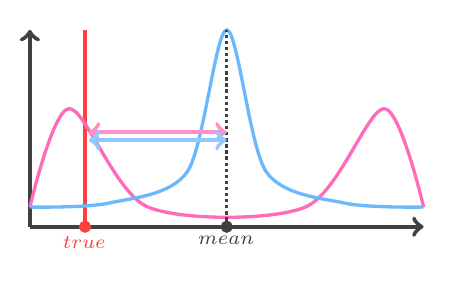
\begin{tikzpicture}[
roundnode/.style={circle, fill=brown!50, very thick, minimum size=11mm},
squarednode/.style={rectangle, fill=dark_cyan!50, very thick, minimum size=10mm},
starnode/.style={regular polygon,regular polygon sides=8, fill=light_blue!66, very thick, minimum size=12mm, inner sep=0},
diamondnode/.style={diamond, fill=pink!66, very thick, minimum size=10mm},]
\draw[black!75, ultra thick, ->] (-5,0.5) -- (0,0.5);
\draw[black!75, ultra thick, ->] (-5,0.5) -- (-5,3);

\draw[red!75, very thick, -] (-4.3,0.5) -- (-4.3,3);
\filldraw[red!75] (-4.3,0.5) circle (2pt) node[anchor=north] {$\DeltaTime^{true}$};

\draw [pink, very thick] plot [smooth, tension=0.5] coordinates { (-5,0.75) (-4.5,2) (-3.5,0.75) (-1.5,0.75) (-0.5,2) (0,0.75)};
\draw [light_blue, very thick] plot [smooth, tension=0.5] coordinates { (-5,0.75) (-4,0.8) (-3,1.2) (-2.5, 3) (-2,1.2) (-1,0.8) (0,0.75)};

\draw[black!75, very thick, densely dotted] (-2.5,0.5) -- (-2.5,3);
\filldraw[black!75] (-2.5,0.5) circle (2pt) node[anchor=north] {$\DeltaTime^{mean}$};

\draw[pink!75, ultra thick, <->] (-4.25,1.7) -- (-2.5,1.7););

\draw[light_blue!75, ultra thick, <->] (-4.25,1.6) -- (-2.5,1.6);

\end{tikzpicture}
\caption{MSE score}\label{fig:MSE_score}
\end{subfigure}
\begin{subfigure}{0.4 \linewidth}
\centering

\definecolor{dark_cyan}{rgb}{0,0.28,0.28}
\definecolor{pink}{rgb}{1,0.42,0.72}
\definecolor{light_blue}{rgb}{0.42,0.72,1}
\definecolor{brown}{rgb}{0.57,0.29,0}

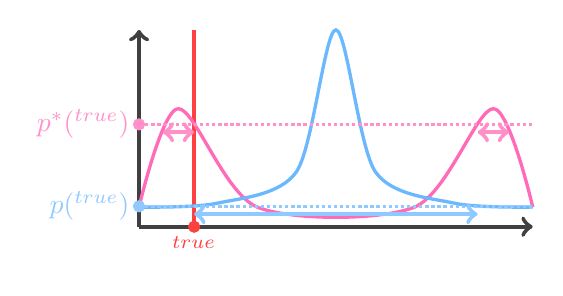
\begin{tikzpicture}[
roundnode/.style={circle, fill=brown!50, very thick, minimum size=11mm},
squarednode/.style={rectangle, fill=dark_cyan!50, very thick, minimum size=10mm},
starnode/.style={regular polygon,regular polygon sides=8, fill=light_blue!66, very thick, minimum size=12mm, inner sep=0},
diamondnode/.style={diamond, fill=pink!66, very thick, minimum size=10mm},]
\draw[black!75, ultra thick, ->] (-5,0.5) -- (0,0.5);
\draw[black!75, ultra thick, ->] (-5,0.5) -- (-5,3);

\draw[red!75, very thick, -] (-4.3,0.5) -- (-4.3,3);
\filldraw[red!75] (-4.3,0.5) circle (2pt) node[anchor=north] {$\DeltaTime^{true}$};

\draw [pink, very thick] plot [smooth, tension=0.5] coordinates { (-5,0.75) (-4.5,2) (-3.5,0.75) (-1.5,0.75) (-0.5,2) (0,0.75)};
\draw [light_blue, very thick] plot [smooth, tension=0.5] coordinates { (-5,0.75) (-4,0.8) (-3,1.2) (-2.5, 3) (-2,1.2) (-1,0.8) (0,0.75)};

\draw[pink!75, very thick, densely dotted] (-5,1.8) -- (0,1.8);
\filldraw[pink!75] (-5,1.8) circle (2pt) node[anchor=east] {$p^*(\DeltaTime^{true})$};
\draw[pink!75, ultra thick, <->] (-4.7,1.7) -- (-4.3,1.7);
\draw[pink!75, ultra thick, <->] (-0.3,1.7) -- (-0.7,1.7);

\draw[light_blue!75, very thick, densely dotted] (-5,0.76) -- (0,0.76);
\filldraw[light_blue!75] (-5,0.76) circle (2pt) node[anchor=east] {$p(\DeltaTime^{true})$};
\draw[light_blue!75, ultra thick, <->] (-4.3,0.66) -- (-0.7,0.66);

\end{tikzpicture}
\caption{\TimeScore}\label{fig:time_score}
\end{subfigure}
\caption{The pink curve is the true time distribution and the blue curve is a uni-modal time distribution.  The value $t^{true}$ is the occurrence time of an event sampled from the true distribution. As it it shows by the arrow the MSE consider that the two distributions have the same quality. In contrast, the \TimeScore estimates that the true distribution is better than the uni-modal distribution}
\end{figure}